
\documentclass[12pt]{article}
\usepackage{geometry} % see geometry.pdf on how to lay out the page. There's lots.
\geometry{a4paper} % or letter or a5paper or ... etc
\usepackage{bm} % see geometry.pdf on how to lay out the page. There's lots.
\usepackage{amsmath}
\usepackage{graphicx}
\usepackage{pdflscape}
\usepackage{subcaption}
\usepackage[round]{natbib}
% \geometry{landscape} % rotated page geometry

% See the ``Article customise'' template for come common customisations

\title{Selective constraints on global plankton dispersal}
\author{B.A. Ward, B.B. Cael, C.R. Young and S. Collins}
\date{} % delete this line to display the current date

%%% BEGIN DOCUMENT
\begin{document}
 

\maketitle


Ecotypes - adapted to different environments - but also many more genotypes.

How evolutionarily stable are these genotypes? Do genetic differences represent stable niche separation?

Observations (Kashtan 2014) suggest very hundreds of subpopulations with millions of years genetic dispersal - hence ecologically meaningful.

Clear(?) succession of genetically distinct subpopulations through time

Key question is how much gene flow between environments/niches???




\textit{``Everything is everywhere, but the environment selects''} \citep{BaasBecking:1934}. \citep[Also Beijerinck: one particular species of bacteria found anywhere on Earth, provided environmental requirements are met...][]{Fenchel:2004} ). Oceanic plankton are sufficiently connected such that all species have the potential to colonise all regions. The community that we see in each location is thus determined by ecological selection. 

\citet{Fenchel:2004}: argue that among small organisms ($<$ 1 mm), this connectivity is facilitated by huge population sizes. At local scale, diversity of small species exceeds that of larger species, but at the global scale, diversity of larger species is greater, driven by endemic differences not seen in smaller organisms. 



\citet{Rossberg:2013}: ``Are there any species smaller than 1 mm?'' [Showed empirical trends and used population model. Need to read again!]


Lagrangian studies have been equivocal. \citet{Hellweger:2014} used an agent-based model to estimate the dispersal and mutation of 100,000 `super-individuals'. They found that realistic rates of mutation were enough to sustain several biogeographic provinces, each with a distinct genetic signature, even in the face of realistic ocean mixing. Genotypes found within these provinces were not distributed globally, which they suggest is in conflict with the notion that “everything is everywhere”. However, it seems likely that the model overestimates the rate at which local diversity is lost by genetic drift \citep[i.e. coalescence??][]{Kingman:1982}, because the modelled population size ($10^{5}$ agents) is so small relative to the true population size ($\sim10^{27}$). [Fixation expected in 273 years, rather than $\sim10^{24}$ years].

\citet{Jonsson:2016} used a (biologically inert) particle tracking model in combination with Dijkstra's `shortest-path algorithm' \citet[][]{Dijkstra:1959} to show that pathways exist to connect the global ocean on timescales of a decade or less. Even though some of the shortest paths are quite unlikely, the huge size of planktonic populations is again invoked to suggest that the pathways should be followed by at least some individuals.  \citet{Jonsson:2016} do not account explicitly for population size, and it remains to be seen how population size and biogeography might affect the predicted patterns of connectivity.


Stochastic approach that accounts for the enormous and variable size of plankton (meta) populations, the potential for stochastic dispersal, and/or a representation of natural selection.

\section{Experiments}

To assess the rate of planktonic dispersal across the global ocean, we developed a model that tracks the abundance of different subpopulations in a globally distributed metapopulation \citep{Cherry:2003}. Throughout the simulation, each of the 60,646 surface grid boxes supports a predefined but spatially variable carrying capacity $\mathbf{N}$. This is derived from the estimated global distribution of 0.6 micron diameter \textit{Prochlorococcus} cells \citep{}. At the beginning of the simulation, a resident subpopulation is assumed to have population frequency of 1 throughout the global ocean. However, this population is replaced with a unique (but ecologically neutral) local subpopulation at 94 `seed locations' distributed more or less evenly around the ocean. 

From this initial condition, the model is integrated for 100 years in discrete time. Every six hours, plankton cells are dispersed by the ocean circulation. We initially considered a scenario where cells are transported exclusively within the surface layer. Every 24 hours the metapopulation is assumed to reproduce. A new metapopulation is drawn at random from a multinomial distribution, with probabilities based on the subpopulation frequencies after dispersal. In regions where a subpopulation is present in high abundance, this stochastic process has no significant effect on the relative abundance of different subpopulations, but it introduces a meaningful chance of local extinction at the boundaries of each subpopulation, or where the overall carrying capacity is low. 

The green line in Figure~\ref{Cumulative} shows the timescales over which the 94 seed subpopulations become connected with the rest of the ocean. Largely in agreement with \citet{Jonsson:2016}, we find that almost 90\% of the surface ocean is connected within a decade. However, we find a much lower value for the median connection times, with a value of just 2.4 years. \textbf{This could be because of increased diffusivities associated with the Eulerian approach used here. But could also be because JW16 discard all indirect shortest paths less than 1 year. Their distribution of 'raw' paths is skewed towards zero (but this could be because longer connections are missed)???}.

\begin{figure*}[htp!]
    \centering
        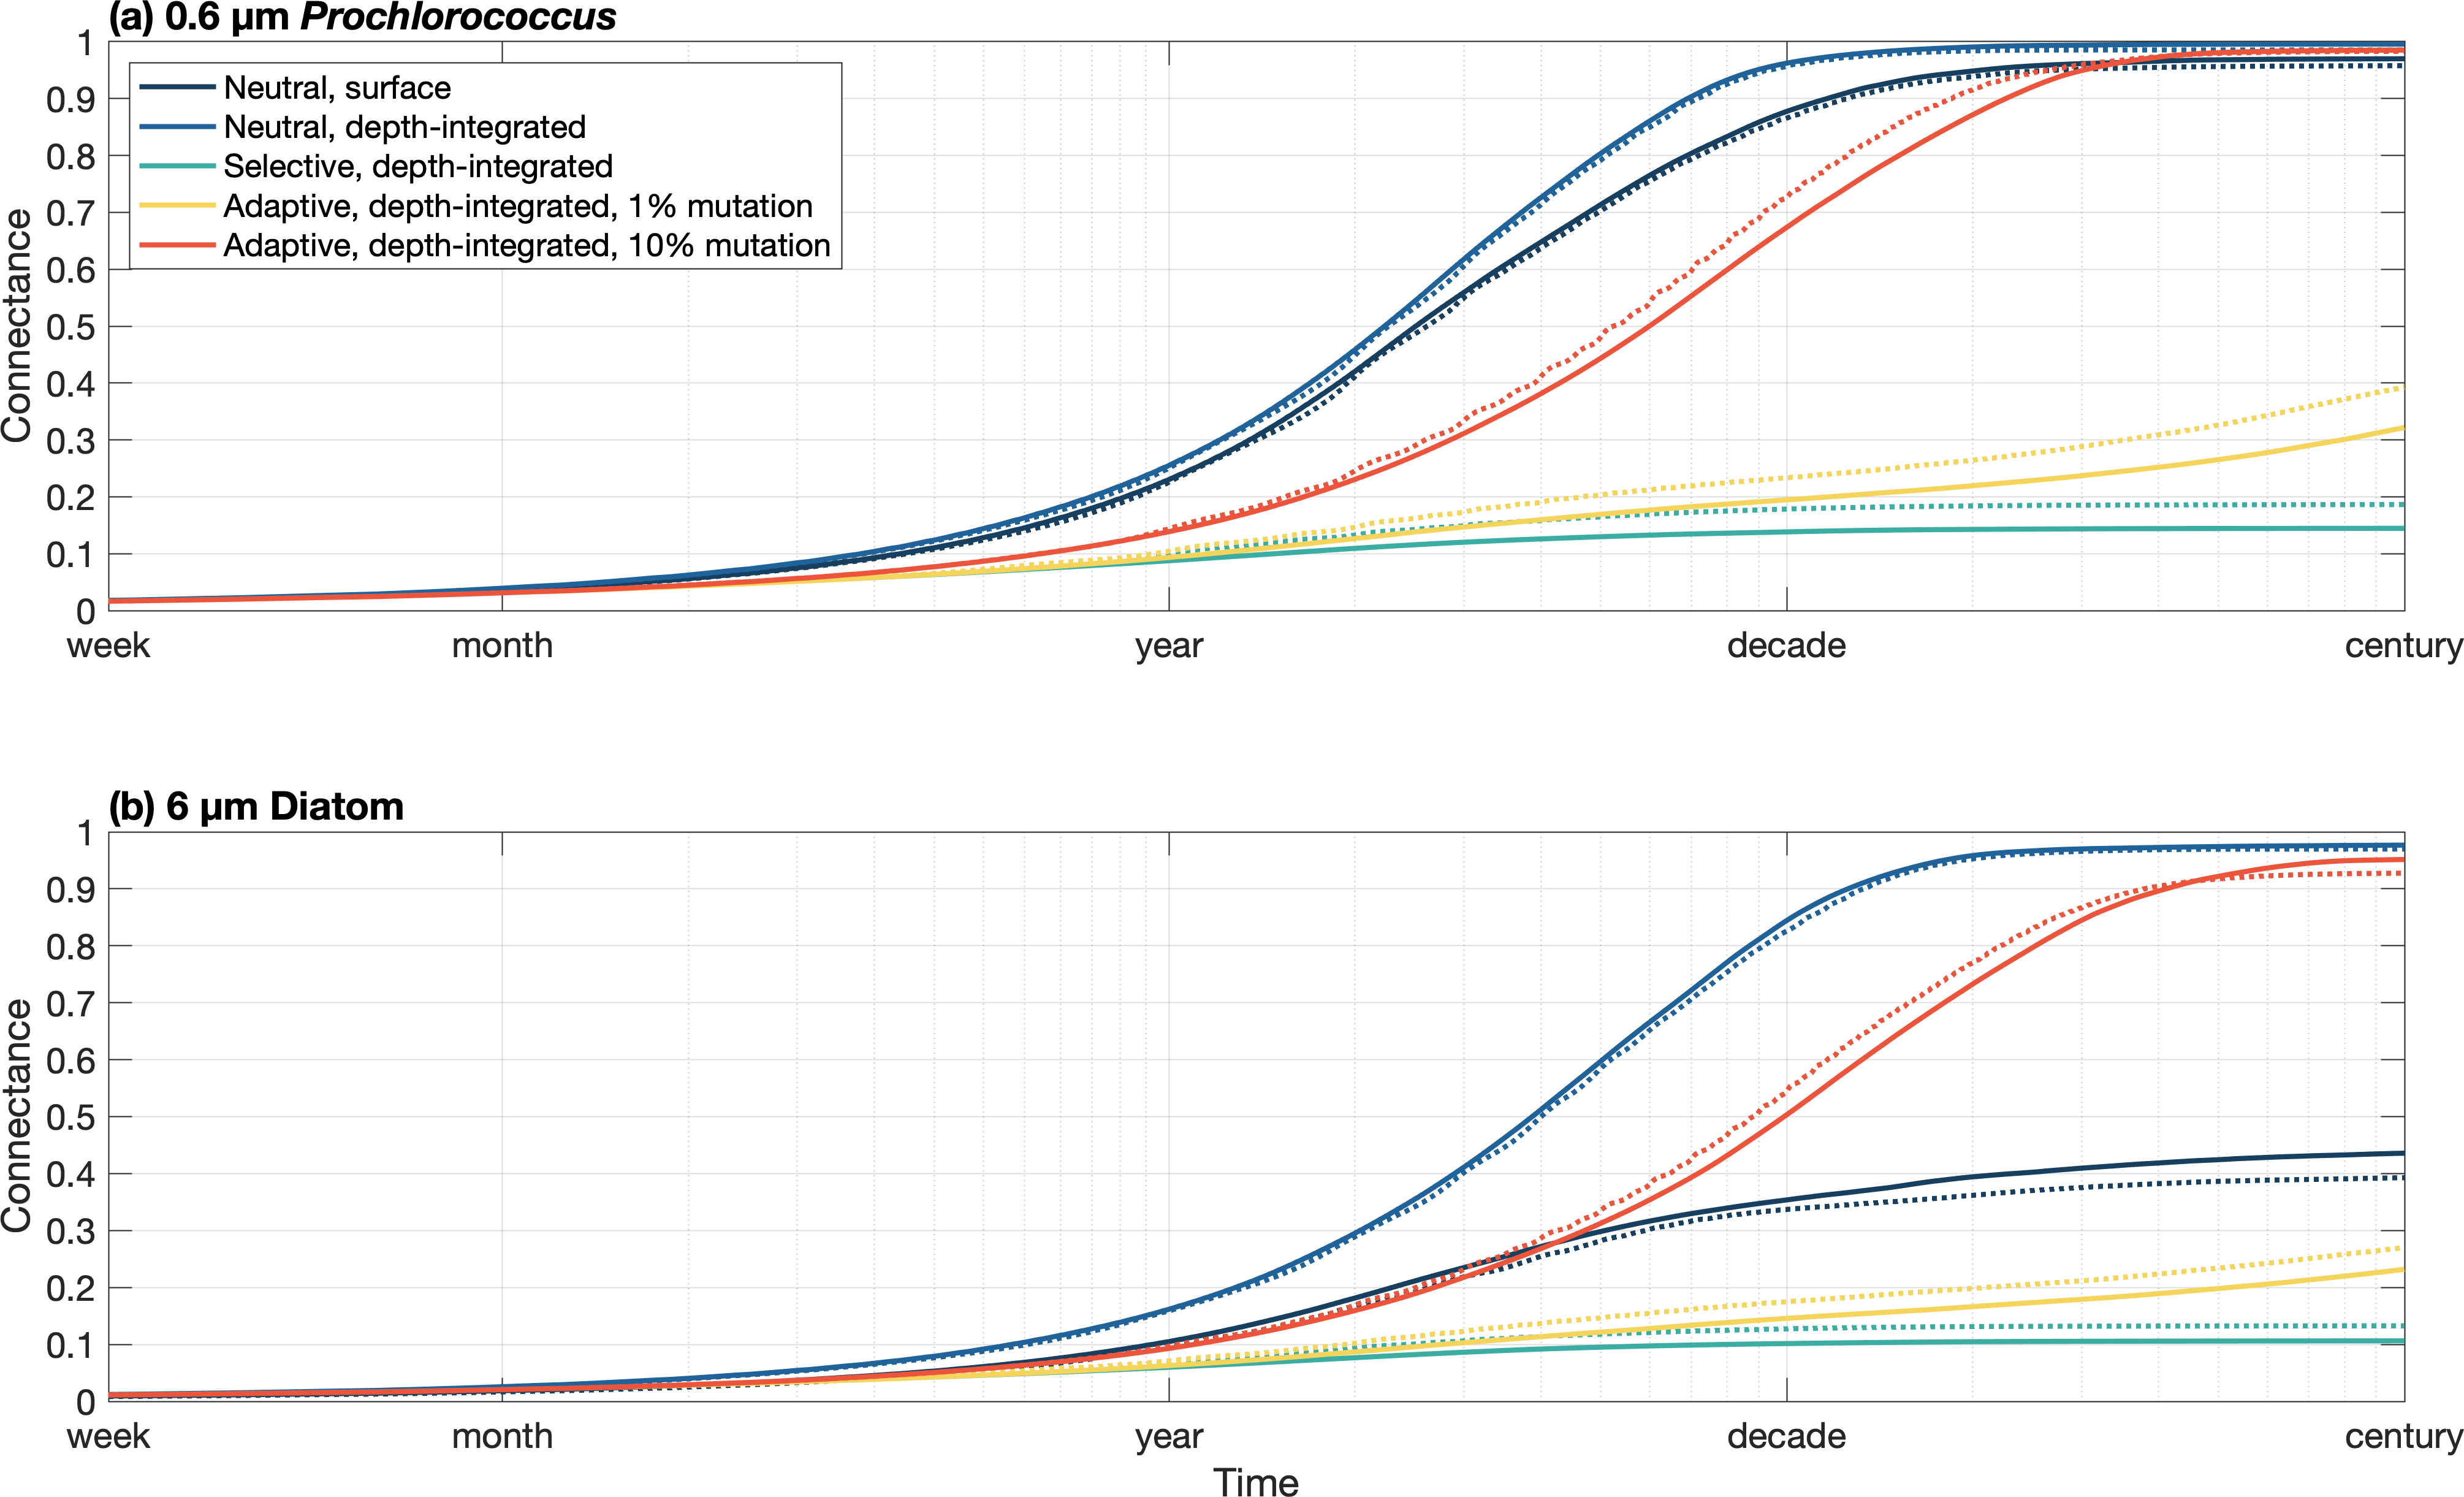
\includegraphics[width=0.5\textwidth]{../Figures/cumulative_connections.png}
\caption{Fraction of connected points between the 94 seed locations and  the rest of the ocean through time}
\label{Cumulative}
\end{figure*}

Global immigration and emigration times are not spatially homogenous, as indicated in Figure~\ref{Connectivity_maps}a. Immigration times (shown as the background colour) suggest that regions between 20 and 60$^\circ$ N and S are the most easily invaded, whereas the equatorial and polar regions appear to be much more resistant  to immigration. Emigration times (shown by the dots) appear to increase either side of a minimum at the equator. 

These patterns are consistent with the surface circulation patterns used to drive the simulation. The equatorial regions are characterised by divergent meridional currents and upwelling. With a consistent efflux of cells being topped up to the carrying capacity, these regions can easily export cells to the rest of the ocean, while remaining resistant to immigration. 

On the other hand, the sub-tropical gyres are characterised by convergent flow and downwelling. Immigrant cells are continually entrained from bordering regions, with a significant loss to resident cells imposed by the constant carrying capacity. These regions are thus easily invaded and are slower to export cells to the rest of the ocean.

The red dots in Figure~\ref{Connectivity_maps}d show that there are `source' regions with slow immigration and fast emigration, and conversely there are `sink' regions with fast immigration and slow emigration.

\begin{figure*}[htp]
        \centering
\begin{subfigure}{.66\textwidth}
        \centering
        \includegraphics[width=1\textwidth]{../Output/neutral_stochastic_static_GUD_X01_surface_transport_341/connection_times_map.png}
    \end{subfigure}%
\\
\begin{subfigure}{.66\textwidth}
        \centering
         \includegraphics[width=1\textwidth]{../Output/neutral_stochastic_static_GUD_X01_weighted_transport_341/connection_times_map.png}
    \end{subfigure}%
    \\
\begin{subfigure}{.66\textwidth}
        \centering
         \includegraphics[width=1\textwidth]{../Output/selective_dispersal_stochastic_static_GUD_X01_weighted_transport_94_mut_0.1/connection_times_map.png}
    \end{subfigure}%
    \\~\\
\begin{subfigure}{.66\textwidth}
        \centering
         \includegraphics[width=1\textwidth]{../Output/selective_dispersal_stochastic_static_GUD_X01_weighted_transport_94_mut_0.1/colorbar.png}
    \end{subfigure}%
    \\
    \caption{Immigration and emigration timescales (years) given (a) surface transport and (b) depth-integrated transport. Unique subpopulations were seeded in each of the 94 locations marked with dots. Emigration times, represented by the coloured dots, are defined as the time taken for each seed subpopulation to disperse to 95\% of all locations). Immigration times, represented by the background colours, are defined as the time taken for 95\% of all seed subpopulations to arrive in each location.Ocean currents and sea surface temperature. The vectors show planktonic transport velocities in the surface-only and depth-integrated cases}
\label{Imm_vs_em}
\end{figure*}

\begin{figure*}[htp]
        \centering
\begin{subfigure}{.66\textwidth}
        \centering
         \includegraphics[width=1\textwidth]{../Output/neutral_stochastic_static_GUD_X17_weighted_transport_341/connection_times_map.png}
    \end{subfigure}%
    \\
\begin{subfigure}{.66\textwidth}
        \centering
         \includegraphics[width=1\textwidth]{../Output/selective_dispersal_stochastic_static_GUD_X17_weighted_transport_94/connection_times_map.png}
    \end{subfigure}%
    \\~\\
\begin{subfigure}{.66\textwidth}
        \centering
         \includegraphics[width=1\textwidth]{../Output/selective_dispersal_stochastic_static_GUD_X17_weighted_transport_94/colorbar.png}
    \end{subfigure}%
    \caption{Immigration and emigration timescales (years) given (a) surface transport and (b) depth-integrated transport. Unique subpopulations were seeded in each of the 94 locations marked with dots. Emigration times, represented by the coloured dots, are defined as the time taken for each seed subpopulation to disperse to 95\% of all locations). Immigration times, represented by the background colours, are defined as the time taken for 95\% of all seed subpopulations to arrive in each location.Ocean currents and sea surface temperature. The vectors show planktonic transport velocities in the surface-only and depth-integrated cases}
\label{Imm_vs_em}
\end{figure*}


\begin{figure*}[t!]
    \centering
        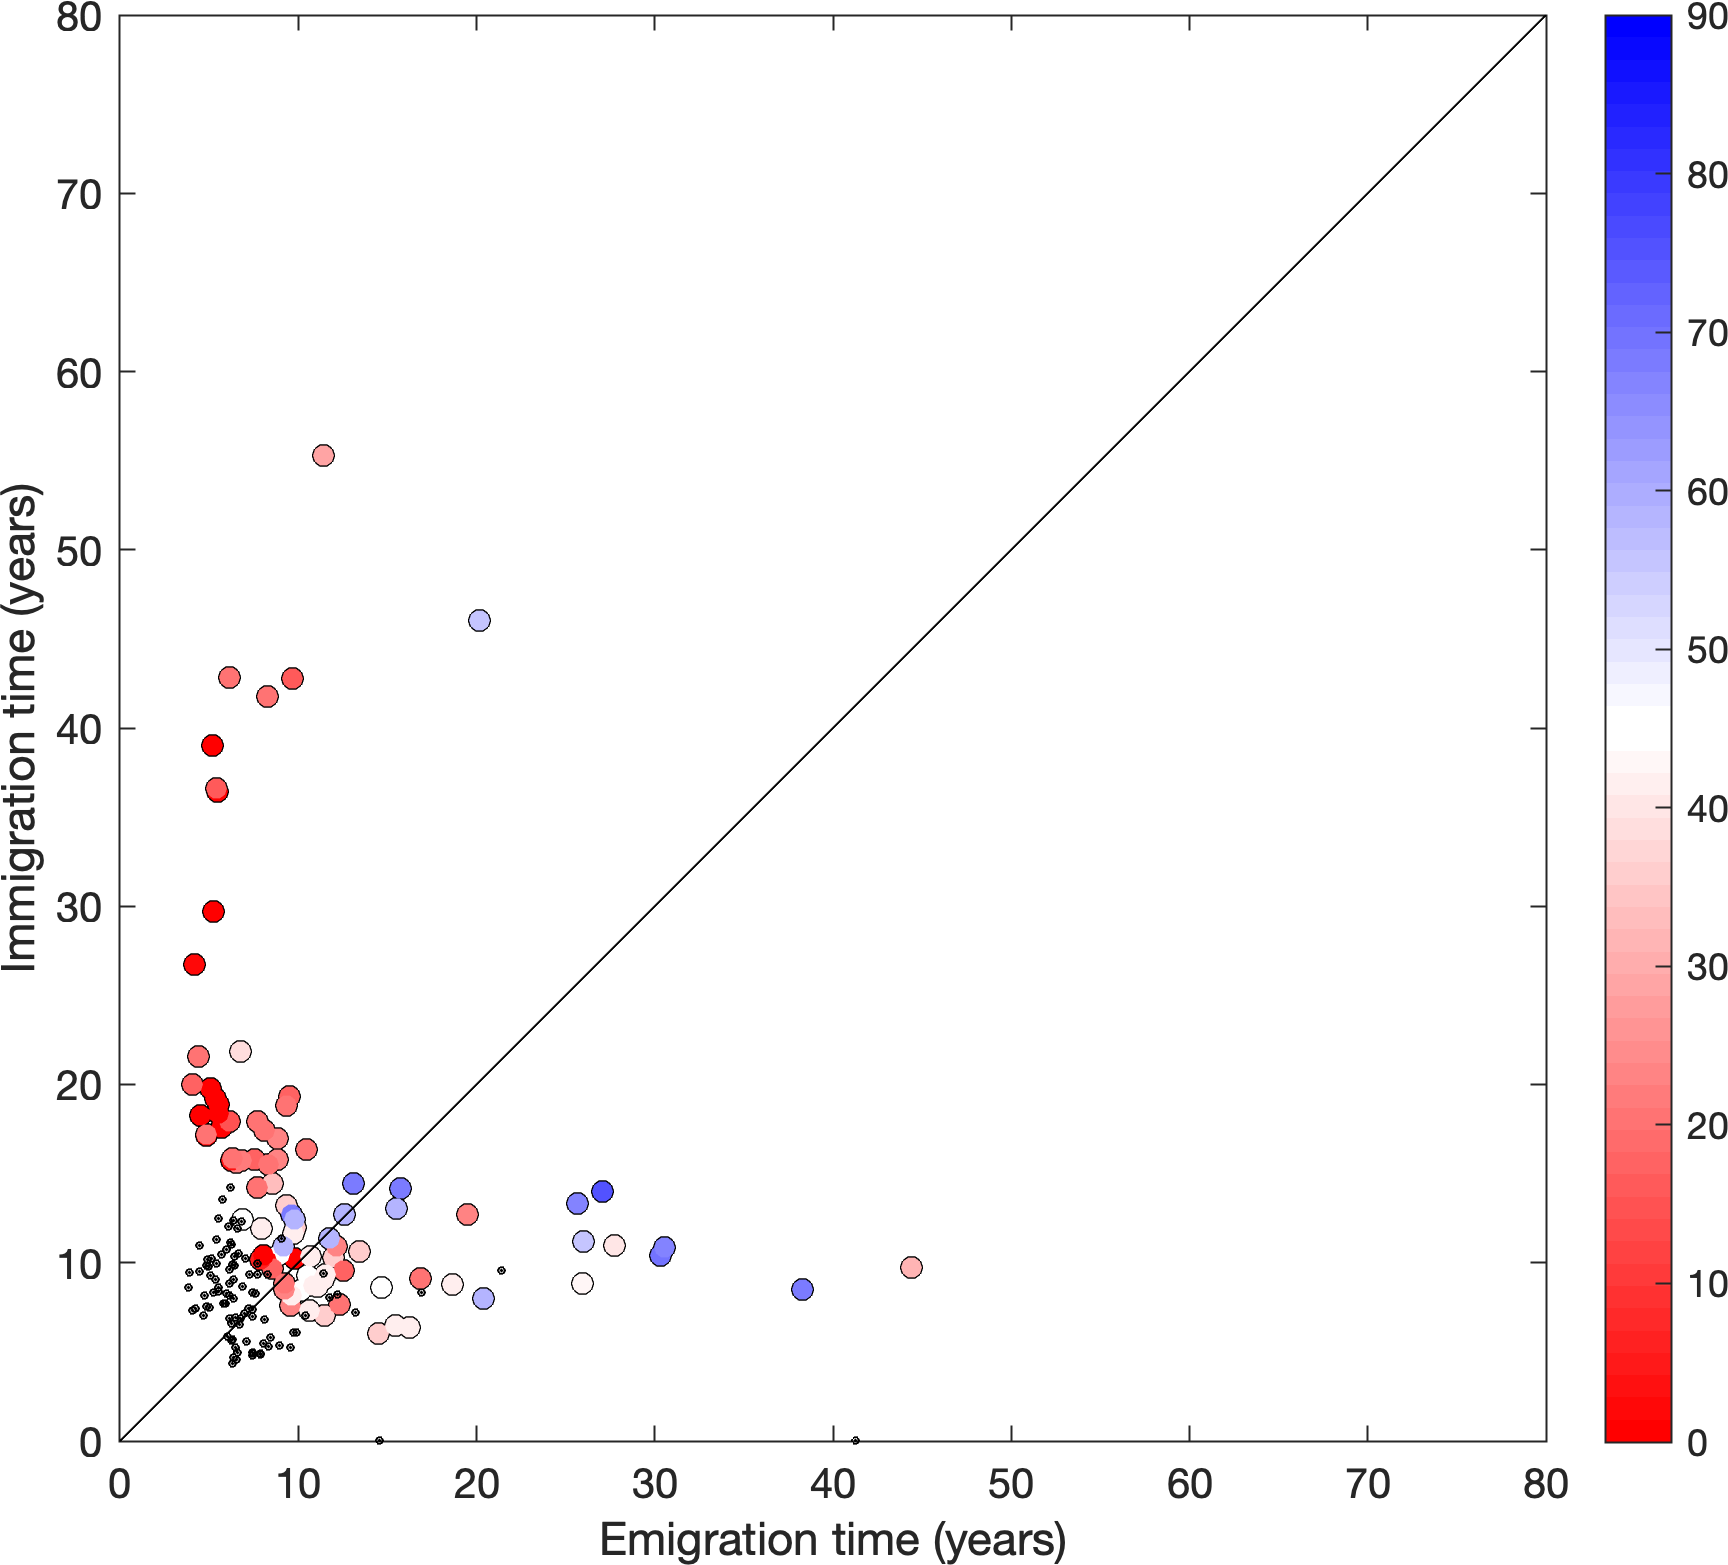
\includegraphics[width=0.6\textwidth]{../Figures/imm_vs_em.png}
    \caption{Immigration vs emigration times (years) at the 94 seed locations. The coloured circles show times from the surface-only case. The colour scale indicates absolute latitude, with low latitude regions clearly characterised by fast emigration and slow immigration, with the opposite true at higher latitudes. The black dots show the same time scales in the depth-integrated case.}
\label{Imm_vs_em}
\end{figure*}



These interpretations of the immigration and emigration times shown in Figure~\ref{Connectivity_maps}a are based on the assumption that transport below the surface layer can be neglected. To test the sensitivity of the model to this assumption, we calculated the depth-integrated horizontal transport of cells across all model layers. This is effectively the depth-integrated horizontal water transport, weighted by the vertical distribution of cellular abundance. The same transport could be achieved by using the full depth-resolved transport, while vertically homogenising each water column at every time step. After this adjustment to the transport component, and with the carrying capacity increased to the depth-integrated cellular abundance, we repeated the initial experiment in exactly the same way. 


The purple line in Figure~\ref{Cumulative} shows that allowing for sub-surface transport markedly decreases the timescales of global plankton dispersal, with a median connection time of 2.1 years, such that more than 97\% of the ocean is connected within a decade. Figure~\ref{Cumulative} shows the change in immigration and emigration times that occurs with the switch from surface to depth-integrated transport. Figure~\ref{Connectivity_maps}b and c shows that the global distribution of immigration and emigration times has decreased everywhere, with the strongest effects in the Indian ocean, where the surface-only simulation suggested that the region was highly resistant to immigration. The blue dots in Figure~\ref{Connectivity_maps}d show that the difference between source and sink regions largely disappears when the depth-integrated transport is considered. 

We next investigated the effect of carrying capacity on the timescales of global dispersal, changing the carrying capacity to the estimated global distribution of 6 micron diameter diatoms \citep{ref}.

\begin{figure*}[t!]
    \centering
    \caption{Immigration and emigration timescales (years) given (a) surface transport and (b) depth-integrated transport. Unique subpopulations were seeded in each of the 94 locations marked with dots. Emigration times, represented by the coloured dots, are defined as the time taken for each seed subpopulation to disperse to 95\% of all locations). Immigration times, represented by the background colours, are defined as the time taken for 95\% of all seed subpopulations to arrive in each location.Ocean currents and sea surface temperature. The vectors show planktonic transport velocities in the surface-only and depth-integrated cases}
\label{Imm_vs_em}
\end{figure*}


The previous experiments have assumed that all subpopulations are equally well-adapted to conditions throughout the entire ocean. We know however that cells show distinct thermal optima that closely reflect their local environment \citep{Thomas:2012}. Such observations suggest that plankton are able to rapidly evolve their thermal tolerance as the are transported across temperature gradients. To account for this, we divided each of the model subpopulations into 77 distinct phenotypes across a range of thermal optima. We initialised the experiment with each subpopulation optimally adapted to its local temperature, but allowed for a small mutational flux between adjacent phenotypes \citep{Beckman:2019}.


\begin{figure*}[t!]
    \centering
    \caption{Immigration and emigration timescales (years) given (a) surface transport and (b) depth-integrated transport. Unique subpopulations were seeded in each of the 94 locations marked with dots. Emigration times, represented by the coloured dots, are defined as the time taken for each seed subpopulation to disperse to 95\% of all locations). Immigration times, represented by the background colours, are defined as the time taken for 95\% of all seed subpopulations to arrive in each location.Ocean currents and sea surface temperature. The vectors show planktonic transport velocities in the surface-only and depth-integrated cases}
\label{Imm_vs_em}
\end{figure*}



% Figure~\ref{Dispersal}a shows the timescales at which a seed population initialised in the Mediterranean Sea reaches the rest of the surface ocean




\section{Methods}


We used the population model to estimate the global dispersal of 341 genotypes, each initialised at unique ``seed locations'' that were distributed approximately evenly around the surface ocean. We also included one additional tracer representing a globally resident species, with a genotype frequency of $\mathbf{p} = 0$ at all seed locations, and 1 throughout the rest of the surface grid.

Under the assumption that all species have equal fitness, the number of individuals $\mathbf{X}$ surviving at each generation is drawn randomly from the local population (after oceanic transport and mutation) with probability equal to the local subpopulation frequency ($\mathbf{p} = \mathbf{X} \mathbf{n}^{-1}$). Under these assumptions, the expected population size in each generation is given by the multinomial distribution, 

\begin{equation}
\label{eqn:mnml}
\mathbf{X}\sim\mathcal{M}(\mathbf{n},\mathbf{p})
\end{equation}

For large $\mathbf{N}$, equation~\ref{eqn:mnml} is reasonably approximated by a normal distribution.

\begin{equation}
\mathbf{X}\approx\mathcal{N}(\boldsymbol{\mu},\boldsymbol{\sigma})
\end{equation}

with $\boldsymbol{\mu}=\mathbf{n}\circ\mathbf{p}$ and $\boldsymbol{\sigma}=\mathbf{n}\circ\mathbf{p}\circ(1-\mathbf{p})$. (Here the `$\circ$' symbol denotes element-wise multiplication.)




The Evolutionary Plankton Metacommunity Dynamics (EPMD) model considers the global distribution of an arbitrary number of planktonic subpopulations distributed across a two-dimensional (latitude and longitude) ocean grid. The probability of survival for each subpopulation in each generation is a function of its relative abundance and its thermal tolerance to its current environmental temperature. Each subpopulation can be assigned a particular thermal optimum, or its survival can be made independent of growth. Plankton cells are circulated in physical space according to a realistic ocean circulation model \ref{}. 



We estimated minimum connectivity times by integrating the model forward from these initial conditions, noting the time at which each genotype first appeared in each grid cell. 

The Evolutionary Plankton Metacommunity Dynamics (EPMD) model considers the global distribution of an arbitrary number of  planktonic subpopulations distributed across a two-dimensional (latitude and longitude) ocean grid. The probability of survival for each subpopulation in each generation is a function of its relative abundance and its thermal tolerance to its current environmental temperature. Each subpopulation can be assigned a particular thermal optimum, or its survival can be made independent of growth. Plankton cells are circulated in physical space according to a realistic ocean circulation model \ref{}. 


\begin{figure}[htp!]
\centering
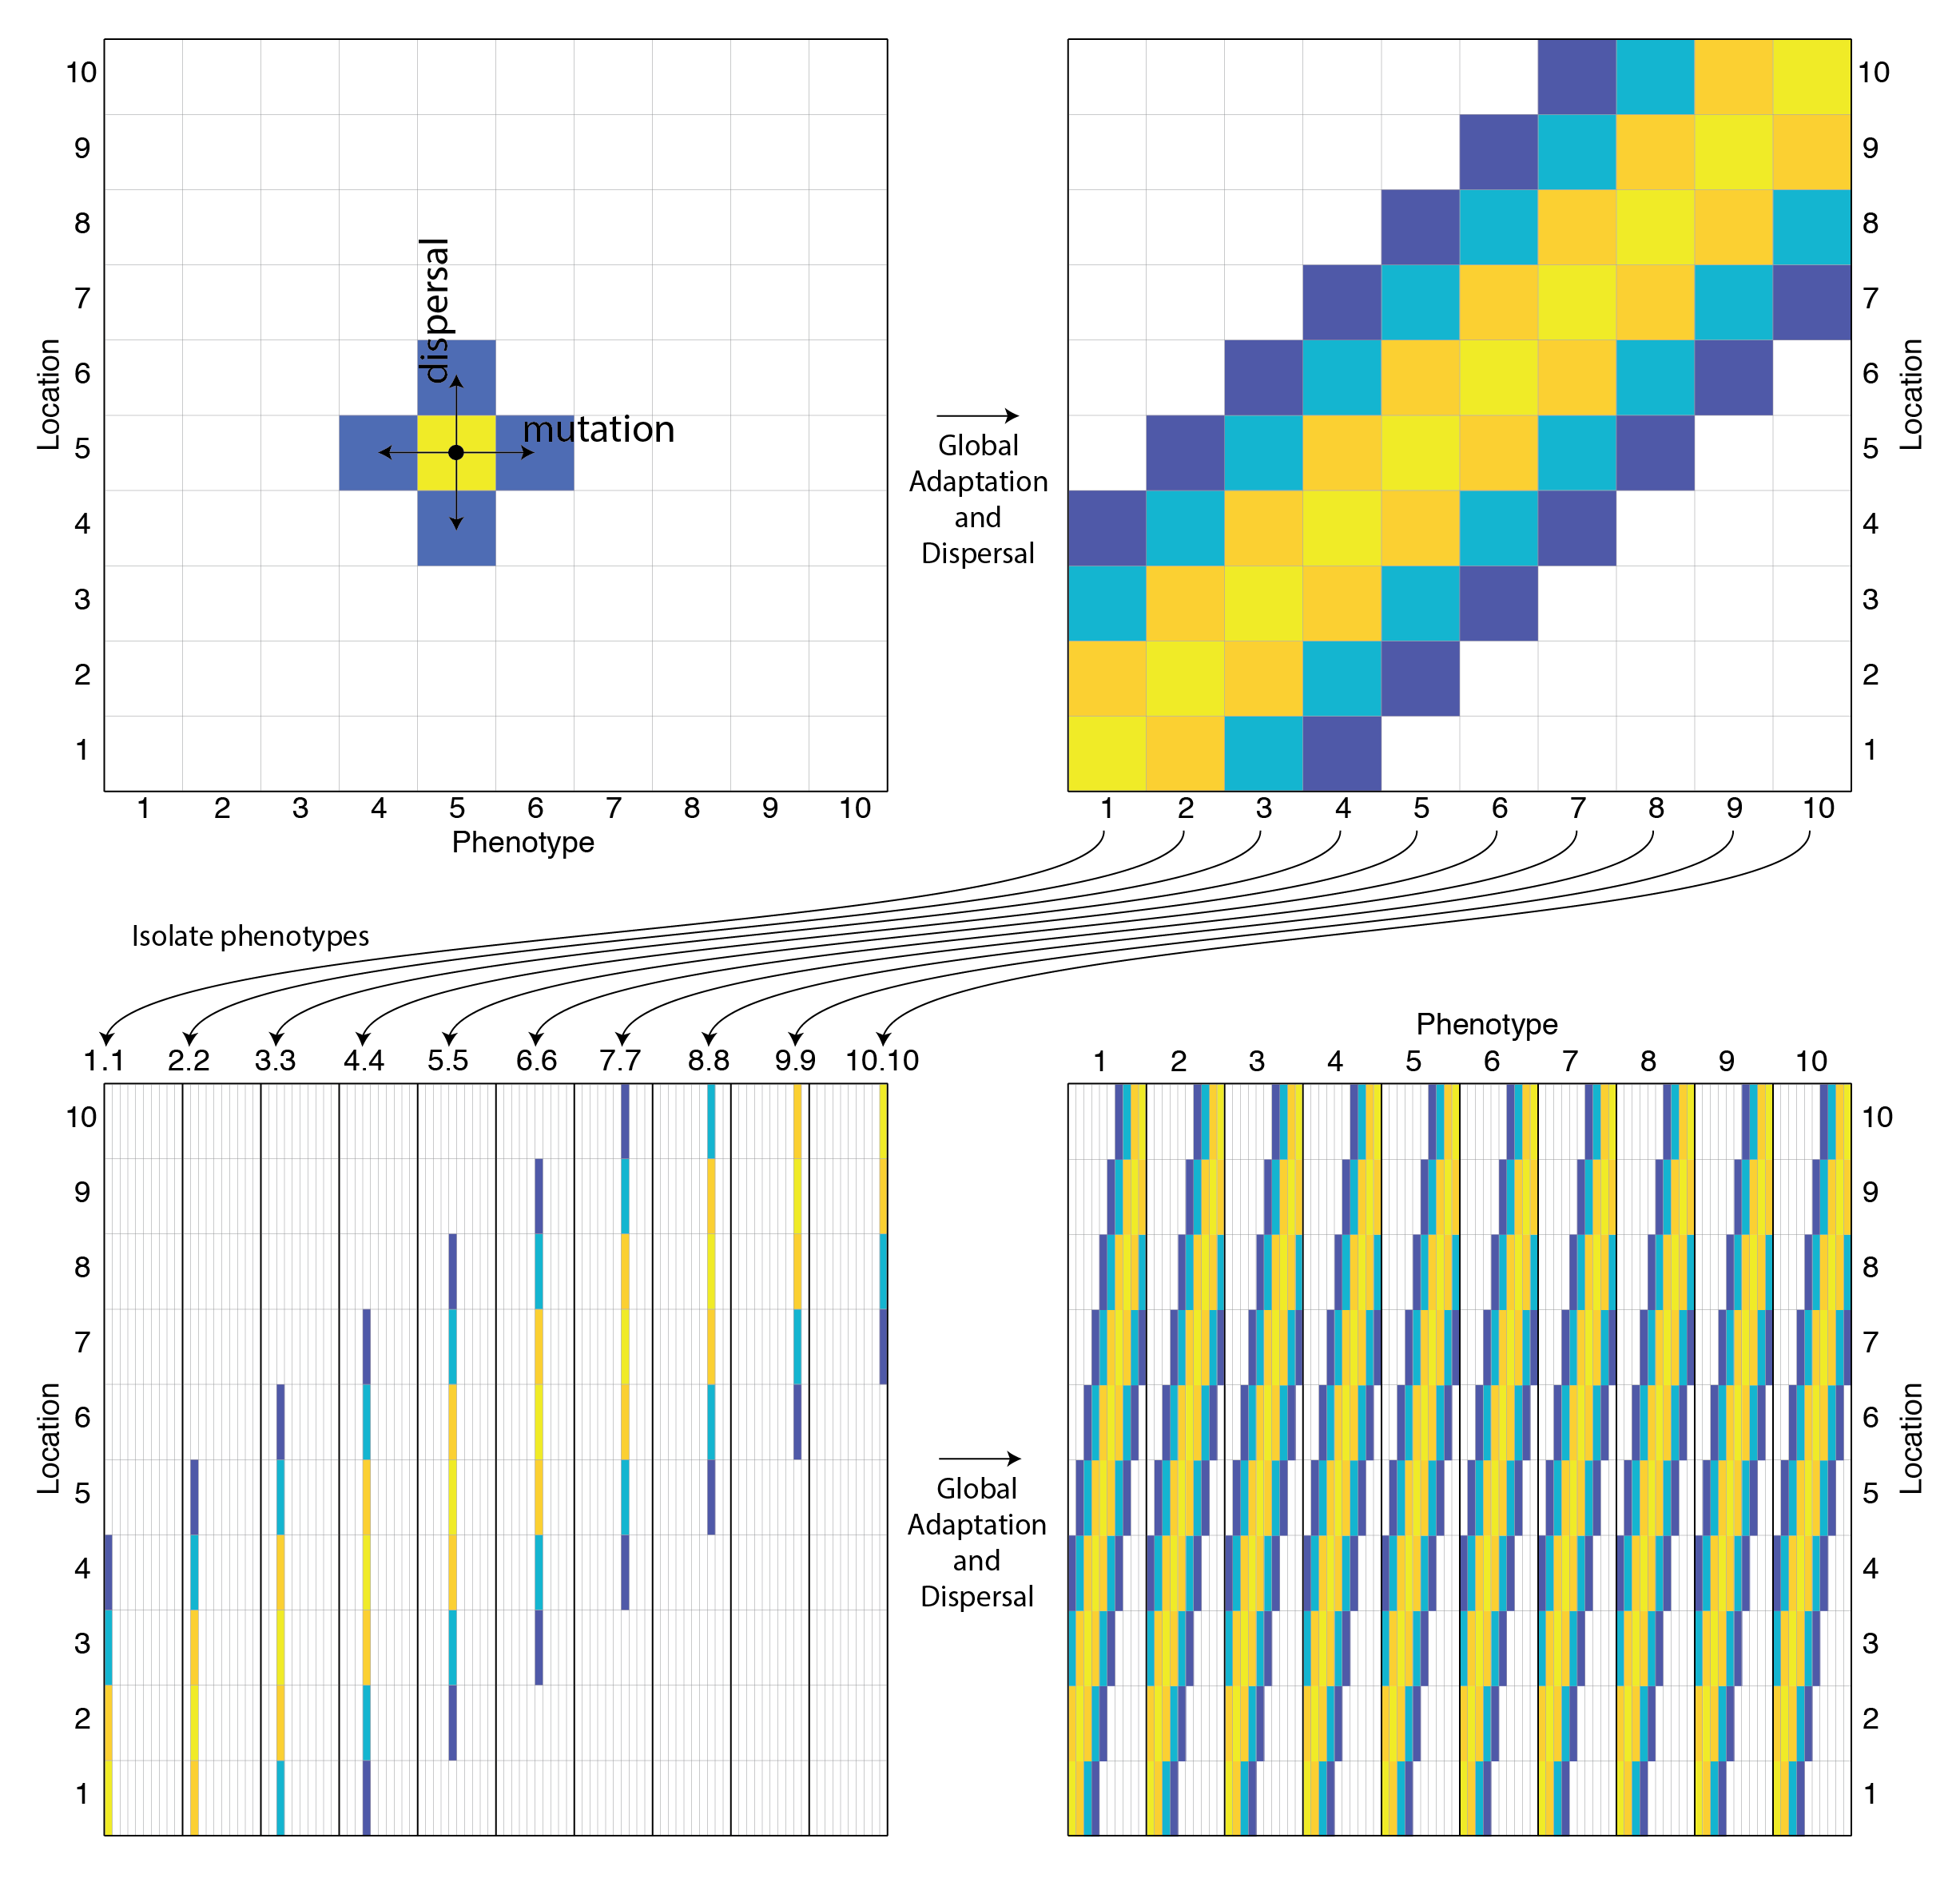
\includegraphics[width=0.8\linewidth]{../Figures/Schematic.png}
\caption{}
\label{Schematic}
\end{figure}


\begin{figure}[htp!]
%%
\begin{subfigure}{0.5\textwidth}
\includegraphics[width=1\linewidth]{../Output/neutral_stochastic_static_GUD_X01_weighted_transport_341/connection_matrix.png}
\end{subfigure}
%%
\begin{subfigure}{0.5\textwidth}
\includegraphics[width=1\linewidth]{../Output/neutral_stochastic_static_GUD_X17_weighted_transport_341/connection_matrix.png}
\end{subfigure}
%%
\caption{}
\label{Schematic}
\end{figure}



\section{Model description}





across $J$ spatial boxes of an ocean general circulation model (GCM). The global abundances of all subpopulations are thus represented in the $[J\times K]$ population matrix.



\subsection*{Physical dispersal}

Plankton cells are transported between grid boxes using a $[J\times J]$ oceanic `transport matrix' $\mathbf{A}$ that describes the transport of neutrally buoyant cells between points in the ocean grid \citep{Khatiwala:2005}. This transport can be written as 

\begin{equation}
\label{ }
\mathbf{T} = \mathbf{A}\mathbf{x}_{t}
\end{equation}

Here $\mathbf{x}$ is the $[J\times K]$ matrix of genotype frequencies in each grid box of the GCM. Each element of the transport matrix $\mathbf{A}$ describes the transport of cells between source boxes (columns) and recipient boxes (rows). The transport matrix was derived from the ``Estimating the Circulation and Climate of the Ocean'' (ECCO) version 4 ocean model \citep{}. It represents physical transport attributable to advection, diffusion and parameterised sub-grid-scale processes in the ocean model. 

\subsection*{Mutation}

Each plankton subpopulation may be assigned a particular phenotype, defined by its thermal optima.

\subsection*{Selection}



Selection can be further incorporated through the selection vector $\mathbf{s}$, that assigns each population in $\mathbf{X}$ a relative fitness of $1+\mathbf{s}$.

\begin{equation}
\label{ }
\mathbf{p} = \frac{\mathbf{\tilde{p}} \circ (1+\mathbf{s}) } {\mathbf{\tilde{p}} \circ (1+\mathbf{s}) + 1 -\mathbf{\tilde{p}}}
\end{equation}

\begin{equation}
s = \exp\bigg[-\Big(\frac{T_{env}-T_{opt}}{w}\Big)^2\bigg]
\end{equation}



%If we model just two genotypes, the expected population size in each generation of the first genotype is given by the binomial distribution, 
%\begin{equation}
%\label{eqn:mnml}
%\mathbf{X_1}\sim\mathcal{B}(\mathbf{n},\mathbf{p_1})
%\end{equation}
%The binomial distribution is also reasonably approximated by a normal distribution for large $\mathbf{N}$. The expected population size of each genotype is then simply $\mathbf{X_2} = \mathbf{N}-\mathbf{X_1}$.


Thermal niche. Seed with n plankton types, each adjusted to a different optimal temperature. How connected are these phenotypes? How does the connectivity depend on population size? on the shape of the thermal niche? Do results compare well with Thomas 2012 or Righetti 2019?







\subsection{Connectivity}






\section{Results}

\subsection{Timescales of dispersal}

Seed subset of ocean regions with one tracer each. Examine time until globally distributed. Dispersal potential increases with local population size.


\begin{figure}[htp!]

\caption{Left-hand side: global abundance distribution of prochlorococcus (top) and diatoms (bottom). Right-hand side: timescales of ocean connectivity for the same two groups. Background colour: shortest timescales over which particles from 95\% of the seed locations (indicated by dots) are expected to have arrived at each point (i.e. immigration timescales). Dots: timescales over which particles from that seed location are expected to have arrived at 95\% of the ocean surface (i.e. emigration timescales).}
\label{connectivity_90_prctile}
\end{figure}



\subsection{Spatial clustering by timescales of connectivity}


\begin{figure}[htp!]

\caption{Pairwise global minimum connectivity and clustering. Upper panel: matrix of the connectivity times between seed locations. Columns of the matrix correspond to source locations (such that row values represent emigration timescales), while rows correspond to target locations (such that column values represent immigration timescales). Lower panel: Clustering of the seed locations on the basis of the average of the immigration and emigration timescales between each location. Coloured boxes in the upper panel indicate clusters defined by the average timescales of connectivity (as shown in the lower panel).}
\label{connectivity_matrices}
\end{figure}








%\subsection{Expected shortest path connectivity}
%The shortest path between the Arctic Ocean and Weddel Sea in the ECCO GCM traverses only 500 grid boxes. It could, in theory, be completed in under two years. However, probability of a single particle following all 500 required steps in sequence is effectively zero (actually 10$^{-662}$). By accounting for the expected waiting time between grid cells, we can come up with a more realistic estimate for the expected journey time of 41 years. This is the average time taken for any particles that do follow the shortest path, accounting for time spent waiting in each grid box.
%Applying the transport matrix until all shortest paths have been followed...
%\begin{equation}
%\label{ }
%\mathbf{B} = \mathbf{A}^n
%\end{equation}




\clearpage 

\appendix

\section{Appendix}

\subsection{Mass conservation correction}

Numerical constraints within the GCM mean that some off-diagonal elements may be negative. To remove these artefacts, negative fluxes out of a box are converted to positive fluxes into the box. If we first define the matrix of negative off-diagonal elements as follows,

\begin{equation}
N_{i,j} = 
\begin{cases}
0 		& \text{if $i=j$ or $A_{i,j}\ge 0$}\\
A_{i,j} 	& \text{if $i\ne j$ and $A_{i,j}<0 $}
\end{cases}
\end{equation}

We first move the off-diagonal negatives to their transpose, changing the sign.

\begin{equation}
\mathbf{B} = \mathbf{A} - \mathbf{N} + ( - \mathbf{N}^\top)
\end{equation}

To conserve mass, changes in the off-diagonals must be compensated by an equivalent change on the diagonals. This is achieved by adding both the row and column sums of the negative off-diagonals to the diagonal. 

\begin{equation}
C_{i i} = B_{i i} + \sum_{j=1}^J N_{i,j} + \sum_{j=1}^J N_{j,i} \text{ (for all $i$)}
\end{equation}

The resultant matrix is positive-definite on the off-diagonals, and conserves mass.

Finally, the transport matrix is converted from a volume flux per time (m$^3$~d$^{-1}$) to a unitless operator; first dividing through by the volume of the recipient cells ($\mathbf{v}$), then multiplying by the selected time step ($\Delta t$), and adding the identity matrix ($\mathbf{I}$).

\begin{equation}
\mathbf{D} = \frac{\mathbf{C}}{\mathbf{v}} \times \Delta t + \mathbf{I}
\end{equation}

\subsection{Seed locations}

Seed locations were identified by iteratively projecting a subdivided rectangular grid onto the surface of a sphere. Surface ocean coordinates from the GCM grid were then mapped onto these points (by shortest euclidean distance in cartesian coordinates). Finally, the 341 unique coordinates were mapped back to their nearest point on the GCM grid. The model was initialised with one tracer for each of these points, with a genotype frequency of $\mathbf{p} = 1$ at the seed location, and zero everywhere else. 


\bibliography{/Users/baw103/GoogleDrive/biblio1}
\bibliographystyle{/Users/baw103/Latex/elsart-harv.bst}
\end{document}













